\section{Evaluation} \label{sec:eval}

We have evaluated our system on a 64-bit Dell server running Ubuntu
server 8.04 with kernel version 3.2.9. We used one Flash based SSD and
one SATA HDD. The SSD is an Intel SSDSA2CW300G3 2.5-inch with 300G
capacity. The SATA disk is a Maxtor 7L250S0 3.5-inch SATA HDD. Its
capacity is 250GB and its rotational speed is 7200 rpm. The code and
benchmark results are publicly available at
https://github.com/brianchenming/mris.

\subsection{Measure drives}

Firstly, we measured the two storage devices used in our benchmarks.
The results we got support our argument that Flash is good in random
I/O while HDD is not bad in sequential I/Os. We formated both devices
using Ext4. We remount devices before each benchmark to make sure that
all disk caches are dropped. The devices were measured using
Filebench~\cite{filebench-web}. Random read and write were measured
using Filebench built-in workloads \texttt{randomread} and
\texttt{randomwrite}; Sequential read and write were measured using
Filebench built-in workloads \texttt{singalstreamread} and
\texttt{singalstreamwrite}.

\begin{figure}[t]
\begin{centering}
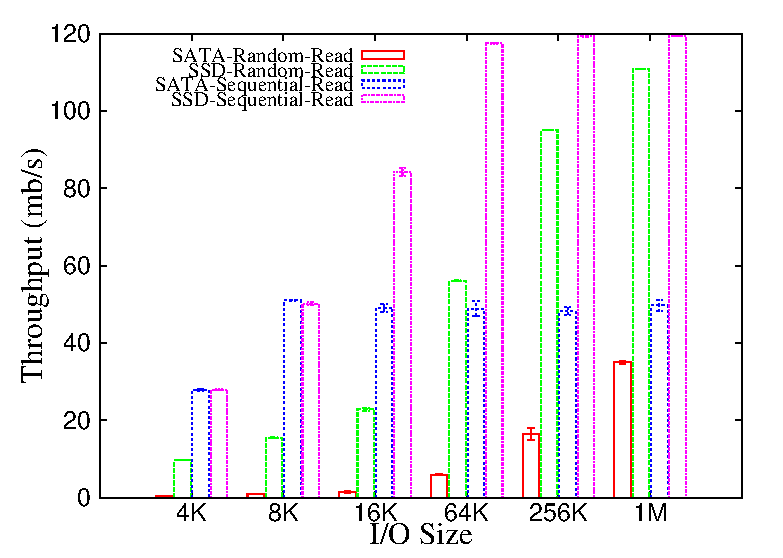
\epsfig{file=figures/ssd_vs_sata_read.eps,width=1.00\linewidth}
\caption{Read performance of SSD and HDD}
\label{fig:driveread}
\end{centering}
\end{figure}

The performance of read operations are presented in
Figure~\ref{fig:driveread}. All benchmarks are performed for 3 times,
and the standard deviation of the 3 runs are shown as error bar in the
figures. The results are stable and most error bars are imperceptible
or negligible. As we can see in Figure~\ref{fig:driveread}, SSD is
much better than that of HDD for random read for small I/O sizes. SSD
is 23.1$\times$ faster than HDD when I/O size is 4K, and 18.4$\times$
faster when I/O size is 8K. However, the speed advantage drops to
8.4$times$ and 4.8$times$ when the I/O size grows to 64K and 256K.
This is because disk head seek happens less frequently as I/O size
increases. Specifically, the HDD read throughput is 0.4mb/s with an
I/O size of 4K. This agrees with the 9ms average read time shown in
the HDD's specification.  

For sequential read, the most interesting observation is that HDD
provided the same throughput as SSD when I/O size is 4K and 8K. HDD
throughput stop grow after 8K, whereas SSD throughput grows until
256K. 8K and 256K are the points when HDD and SSD achieve their
respective maximum bandwidth.

\begin{figure}[t]
\begin{centering}
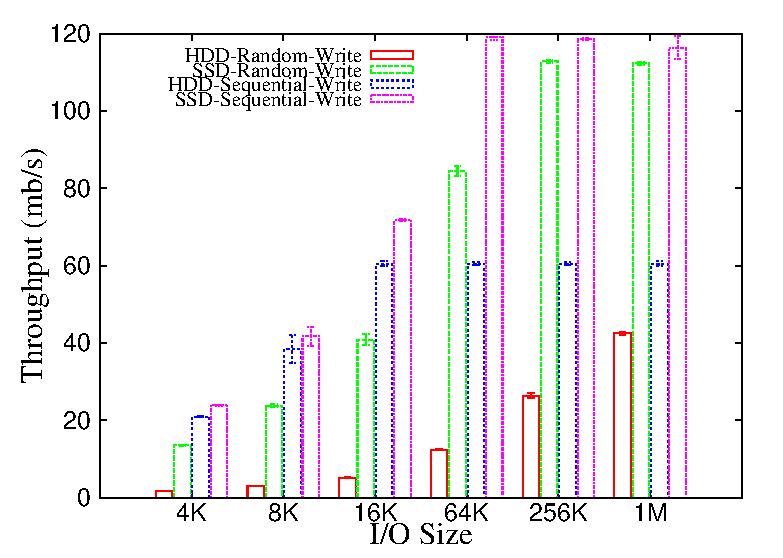
\epsfig{file=figures/ssd_vs_sata_write.eps,width=1.00\linewidth}
\caption{Write performance of SSD and HDD}
\label{fig:drivewrite}
\end{centering}
\end{figure}

The performances of write operations are presented in
Figure~\ref{fig:drivewrite}. They present similar trend as of read.
When I/O size is small (i.e. 4K, 8k, or 16k), SSD performs much better
than HDD for random write, but their performance have no significant
difference for sequential write. When I/O size becomes large,
throughput of both drives are capped by their maximum bandwidth.
However, we noticed that HDD performs better for write than for read.
This is because the HDD has a 16MB internal cache, which is more
helpful for write than for read. 

Above-mentioned results will serve as baselines of throughput for our
further benchmarking. They also validate our design premise that SSD
performs much better than HDD for random I/Os and HDD performs well
for sequential I/Os.

\subsection{Wikipedia Image Workload}

\begin{figure}[t]
\begin{centering}
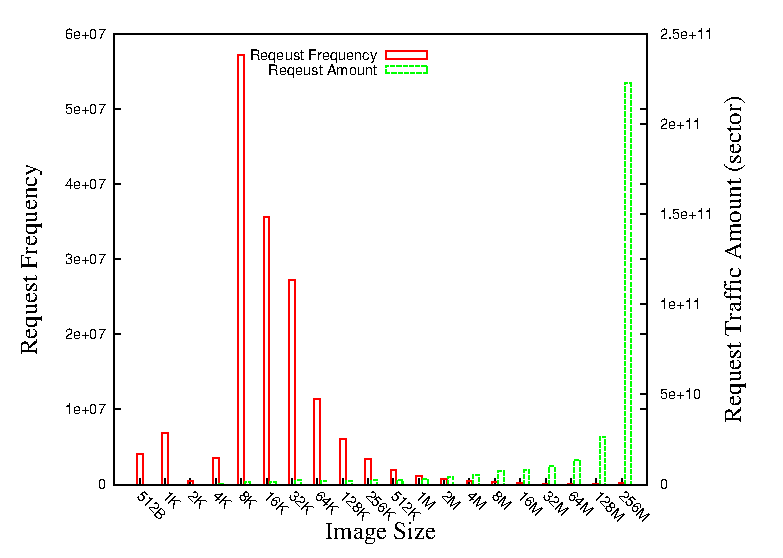
\epsfig{file=figures/wiki-image.eps,width=1.00\linewidth}
\caption{Image Requests to Wikipedia of January 2012}
\label{fig:wikiimage}
\end{centering}
\end{figure}

To study the size-tiered property in workloads, we analyzed the
requests of images made to Wikipedia site.  Wikipedia is the #5
website in the world~\cite{wikipedia-web}, serving 492 million people
every month~\cite{wikipedia-foundation}. It can reflect workloads of
many large websites.

Figure~\ref{fig:wikiimage} presents the requests of images made in
January 2012. They are extraced from request log files, which are
available at
http://dumps.wikimedia.org/other/pagecounts-raw/2012/2012-01/. We
extract requests of objects with a suffix of jpg, png, or gif, then
round up their sizes into power of 2. The frequency of images of
different sizes is counted and plotted in Figure~\ref{fig:wikiimage}.
All images larger than 256M is counted in the 256M bin. The first
observation from Figure~\ref{fig:wikiimage} is that the request image
of different sizes vary widely.  Particularly, images of sizes between
$(4, 64]$ KB are most popular. They sum to 81.58\% of the total number
of image requests. Moreover, 94.57\% of the requests are for images
smaller than or equal to 128KB. Despite the fact that small images
(<=128KB) are the absolute majority in term of request numbers, the
traffic (size$\times$frequency) introduced by them is just 2.96\% of
the total. Although not all the requests make their way to the storage
layer because of memory cache (such as Memcached~\cite{memcached}).
This salient size-tiered property of requests still makes size-tiered
storage a close match for multi-resolution image workloads.

\subsection{MRIS Write}

%The drives were formatted using ext2, whereas fig:drivewrite was
%using ext4. This should not have happened. We need to redo one of the
%two sets of benchmarks in the future.

We now show micro benchmark results on simple workloads of sequential
and random write of multi-resolution images. Multi-resolution images
of the same content are often created from a common source. Therefore,
they are inserted into the image store at the same time. For example,
In Facebook's Haystack~\cite{beaver2010finding}, four resolutions,
thumbnail, small, medium, and large, are created from each image
uploaded by customers. As most images are in compressed format, we
emulate the workload of writing MRI by inserting groups of random
objects into MRIS with compression disabled. To be simple, each group
consists of two objects, both of which are random strings. One of the
two objects is 8KB large representing a small image, whereas the other
is 128KB large representing a large image. The SizeThreshold is set to
128KB, so that the large one will be stored in LargeSpace.

\begin{table}[t]
{\footnotesize
\centering
\begin{tabular}{c|c|c|}
\cline{2-5}
\cline{2-5}
  Setup & \multicolumn{2}{c} Placement of Objects \\ 
   Name & Small (in SSTable) & Large (in LargeSpace) \\ \cline{1-3}
  SSD & SSD & SSD \\
  Hybrid & SSD & HDD \\
  SATA & HDD & HDD \\ \cline{1-3}
  \end{tabular}
}
 \caption{Setups For Benchmarking. The three setups differ in the
 places objects are stored.}
\label{tbl:setups}
\end{table}

Figure~\ref{fig:mriswrite} presents the results of the workload of
inserting 10,000 groups of objects into MRIS. We experimented the
workload on three different setups in Table~\ref{tbl:setups}. The
groups were inserted in random and sequential ways considering the
order of the key of objects. For ops/sec of random insertion, SSD is
28\% faster than SATA and Hybrid is 8\% faster than SATA. Considering
only SSD and SATA, the speedup of SSD is much lower than that shown in
Figure~\ref{fig:drivewrite}. This is because of the Memtable and the
log-structured feature of MRIS, which turns many random writes into
fewer large sequential write. As we can see in
Figure~\ref{fig:drivewrite}, SSD is only slightly faster than SATA
when it is for sequential write of 4K I/O size. Therefore, a slow
speedup of insertion is reasonable.

For sequential insertion, SSD is 26\% faster than SATA and Hybrid is
just 3\% faster than SATA. This is because sequential insertion causes
less compactions than random insertion, which reduce the overall
number of I/Os.  Compations merge multiple sorted SSTable into one
larger sorted SSTable. When key/value pairs are inserted sequentially,
no merge is necessary because all SSTable have no overlapping keys.
This also explains why sequential insertion is significantly faster
than random insertion for all the three setups (41\%, 38\%, and 45\%
faster for SSD, Hybrid, and SATA). 

\NOTE{Ming}{I really should have recorded the number of compactions
happened during the Benchmarking. I will probably do it in several
days}

% How fdatasync determines which I/O size to use? We will have to
% double check the I/O size. LevelDB has an internal block size
% defaults to 4KB, but that is not necessarily the I/O size.

% LevelDB writes SSTable using mmap and fdatasync. It is better if we
% can get some basic drive benchmarks using mmap in the future.

Figure~\ref{fig:mriswrite} (b) also shows throughput in term of
mb/sec.  However, the speed-up ratio of mb/sec is almost identical to
that of ops/sec (differ in less than 0.1\%). This is what we are
expecting because the average size of an operation is the same among
all setups. We will only show ops/sec in folloing throughput figures.

\begin{figure}[t]
  \centering
  \begin{minipage}[c]{\linewidth}
    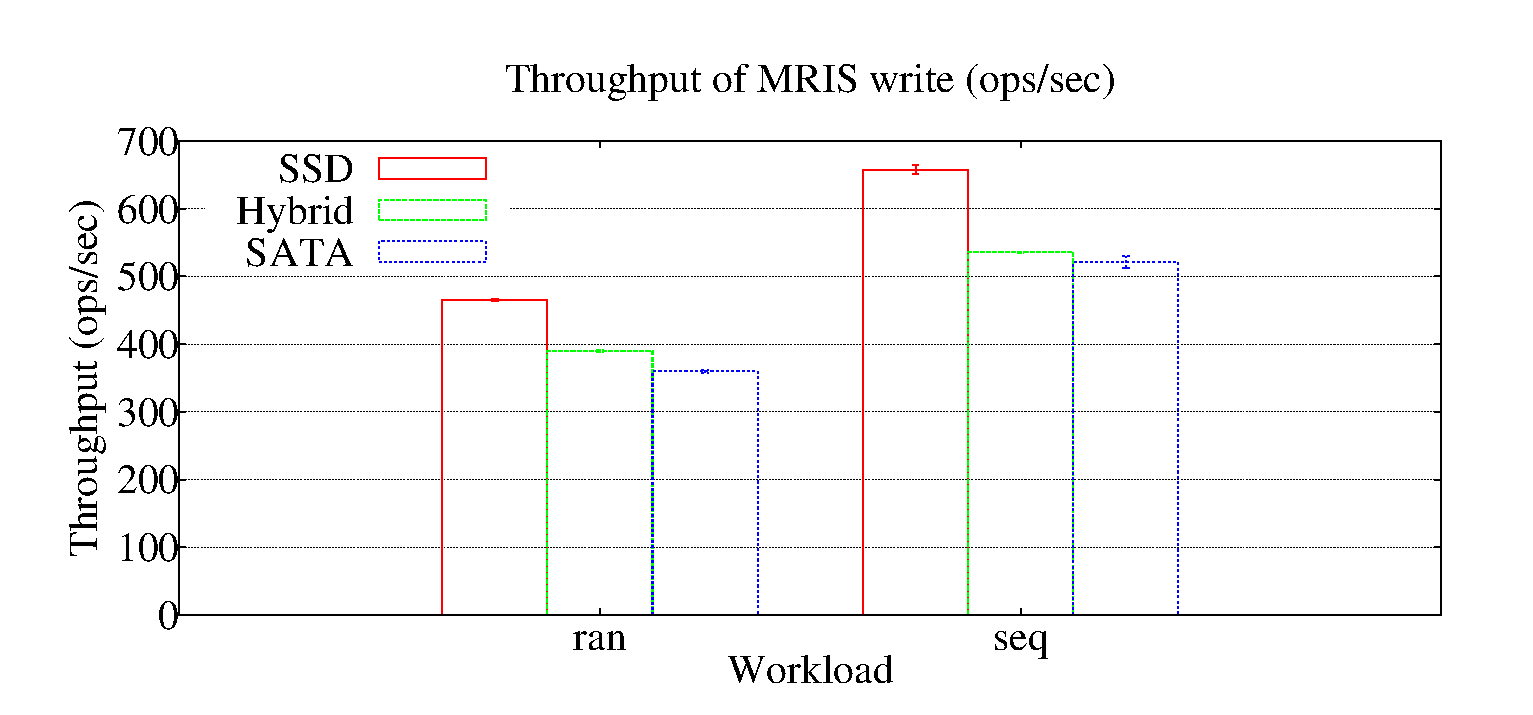
\epsfig{file=figures/mris-write-ops.eps,width=1.00\linewidth}
    \centerline{(a) Objects written per second}\medskip
  \end{minipage}
  \begin{minipage}[c]{\linewidth}
    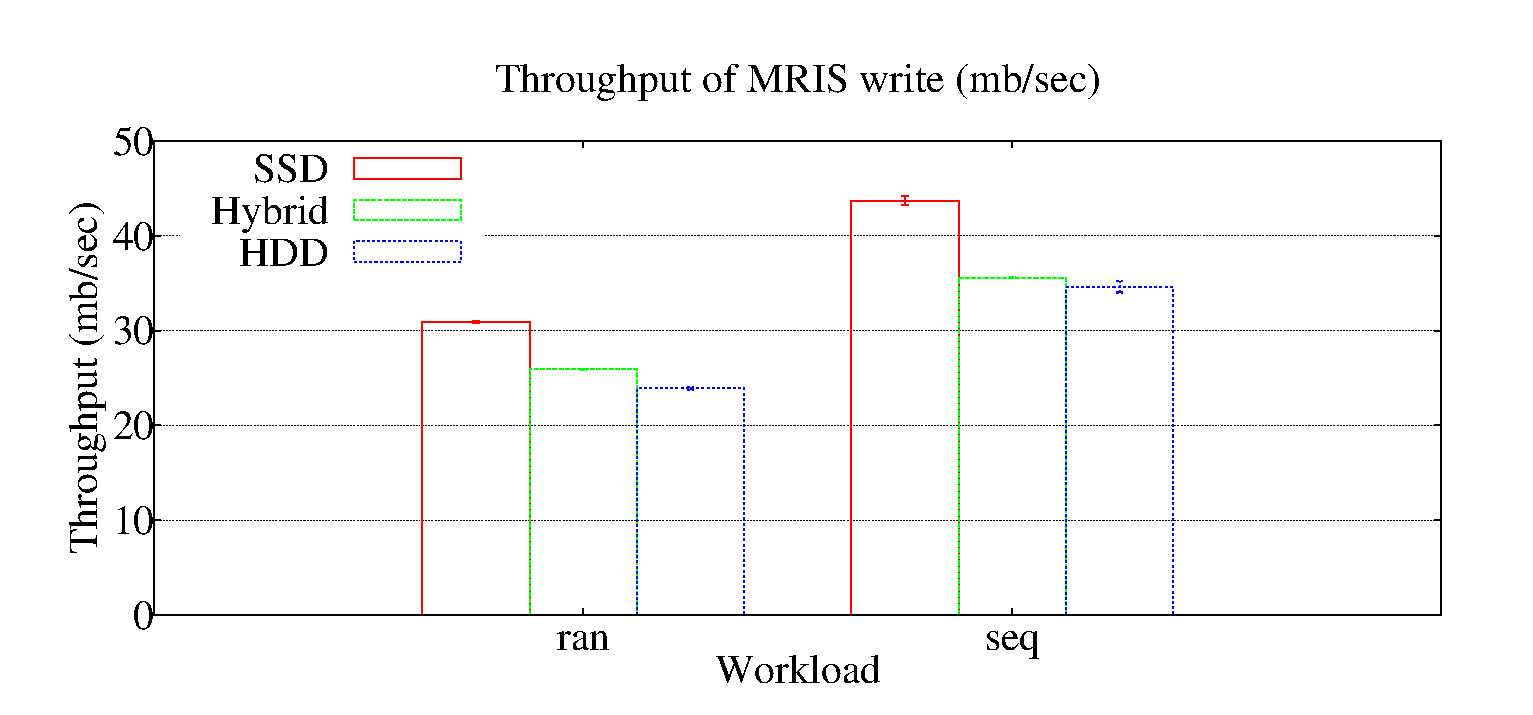
\epsfig{file=figures/mris-write-thput.eps,width=1.00\linewidth}
    \centerline{(b) MB written per second}\medskip
  \end{minipage}
  \caption{Write performance of MRIS.}
  \label{fig:mriswrite}
\end{figure}

\subsection{Facebook Workloads}

1. 17 of Ran R on three setups

2. RR workload of different ratios on hybrid.

%%%%%%%%%%%%%%%%%%%%%%%%%%%%%%%%%%%%%%%%%%%%%%%%%%%%%%%%%%%%%%%%%%%%%%%%%%%%%%
%% For Emacs:
% Local variables:
% fill-column: 70
% End:
%%%%%%%%%%%%%%%%%%%%%%%%%%%%%%%%%%%%%%%%%%%%%%%%%%%%%%%%%%%%%%%%%%%%%%%%%%%%%%
%% For Vim:
% vim:textwidth=70 noai nocin nosi
%%%%%%%%%%%%%%%%%%%%%%%%%%%%%%%%%%%%%%%%%%%%%%%%%%%%%%%%%%%%%%%%%%%%%%%%%%%%%%
% LocalWords:  
